% \section{TODO: FIND NAME}


\begin{frame}[c]{Hi-C Contact Matrix}
    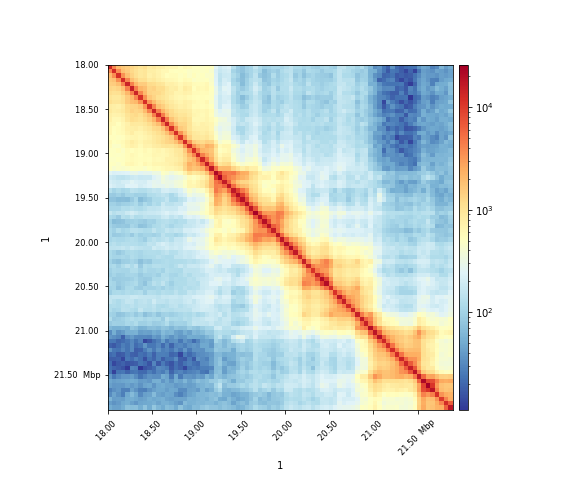
\includegraphics[scale=0.5, trim=50 45 50 30,clip]{c_50kb}
\end{frame}

% \begin{frame}[c]{Enhancer Promoter Interaction}
%                                 % trim = left bottom right top
%     \only<-1>{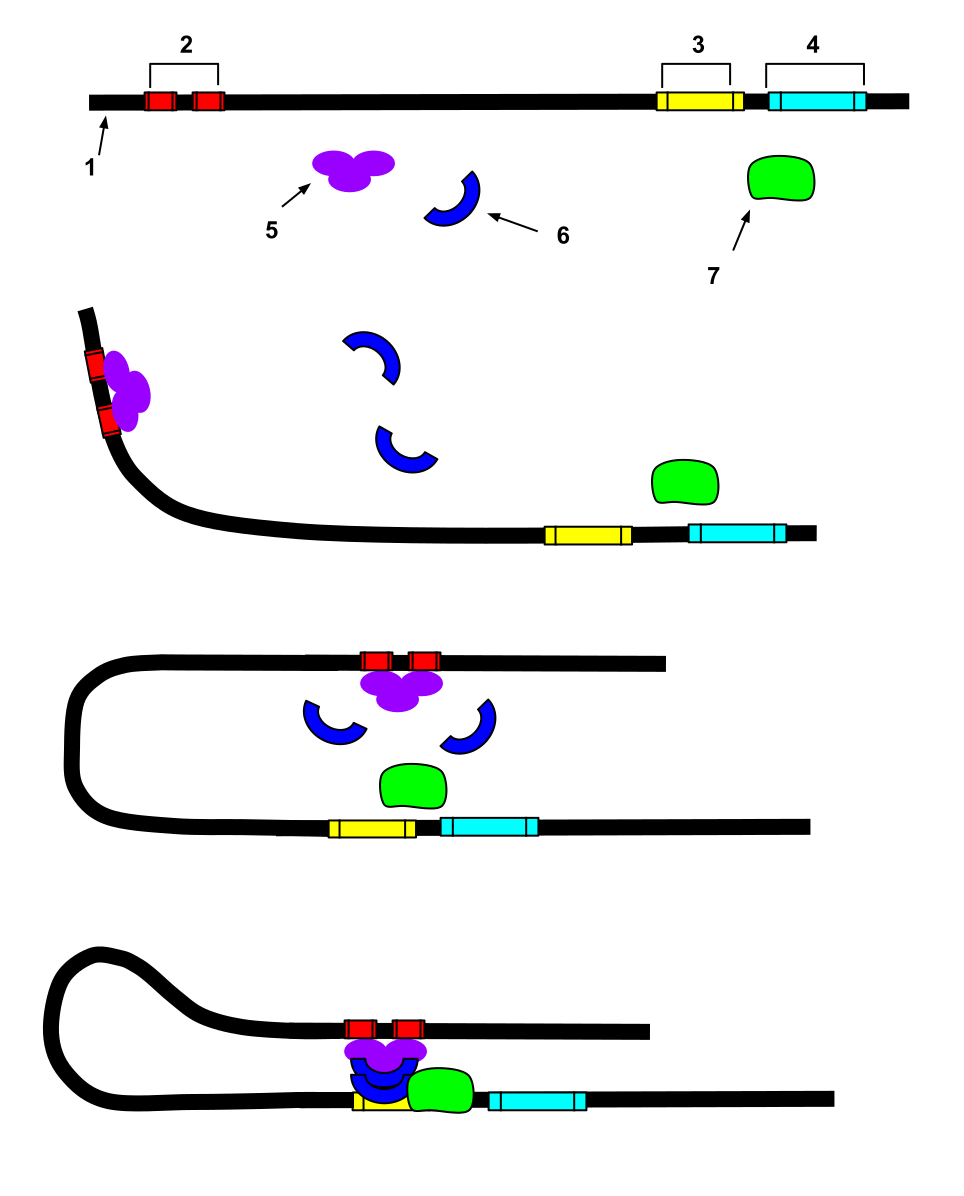
\includegraphics[scale=0.33, trim=0 650 0 0, clip]{Enhancer_Nucleotide_Sequence}}
%     \only<2->{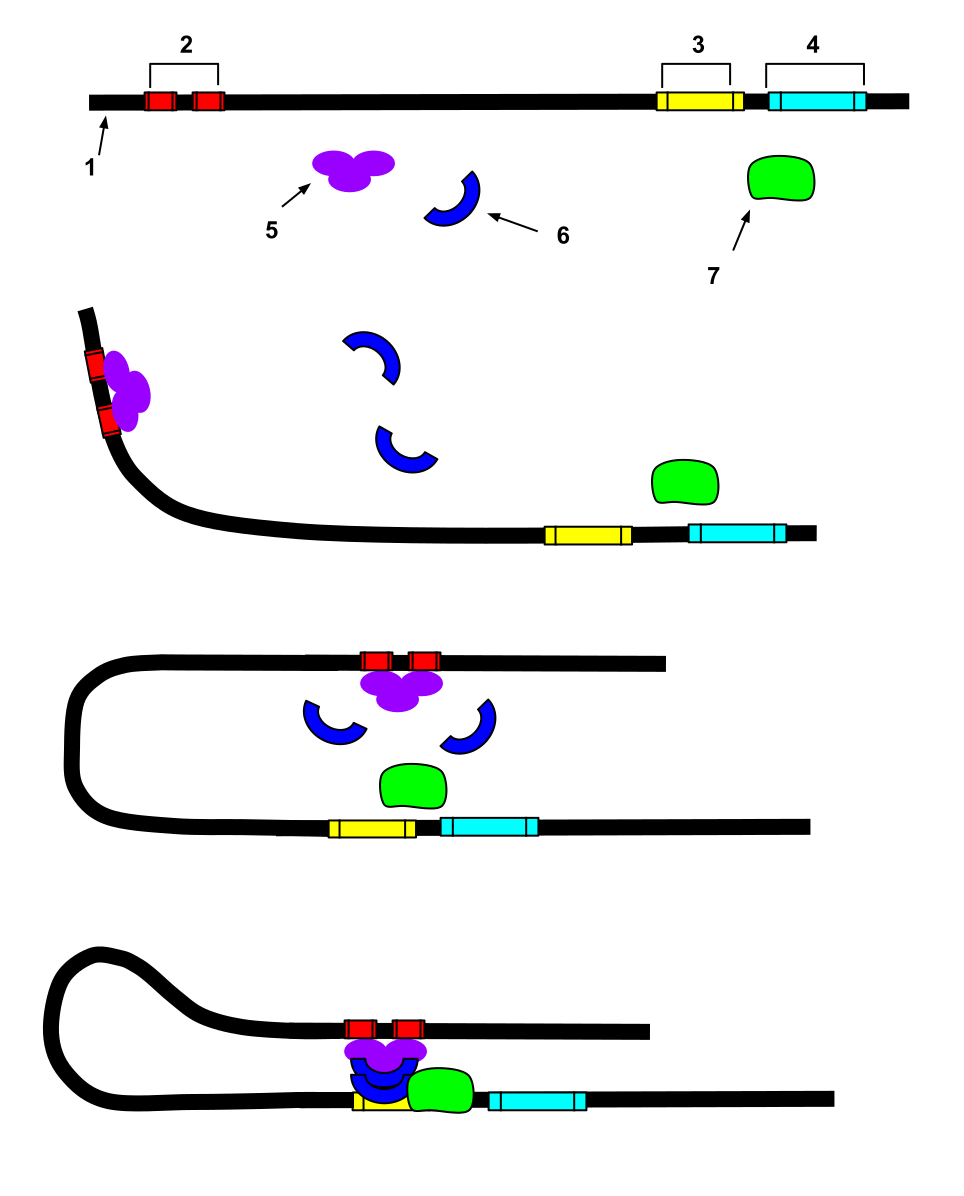
\includegraphics[scale=0.33, trim=0 70 0 580, clip]{Enhancer_Nucleotide_Sequence}}
%     Image adapted from \cite{figenhancers}.
%
%     % Seen here is a four step diagram depicting the usage of an enhancer.
%     % Within this DNA sequence, protein(s) known as transcription factor(s)
%     % bind to the enhancer and increase the activity of the promoter.
%     % 1 DNA
%     % 2 Enhancer
%     % 3 Promoter
%     % 4 Gene
%     % 5 Transcription Activator Protein
%     % 6 Mediator Protein
%     % 7 RNA Polymerase
%
%
%     % - Explain workings of enhancers and promoters in short
%     % - it is relevant for them to have spatial proximity
%     % - Commonly the search for enhancer-promoter pairs
%     %   happens only locally (1 Mbp up- and downstream)
%     % -
% \end{frame}


% \begin{frame}[c]{Chromatin}
%     \only<1>
%
%     {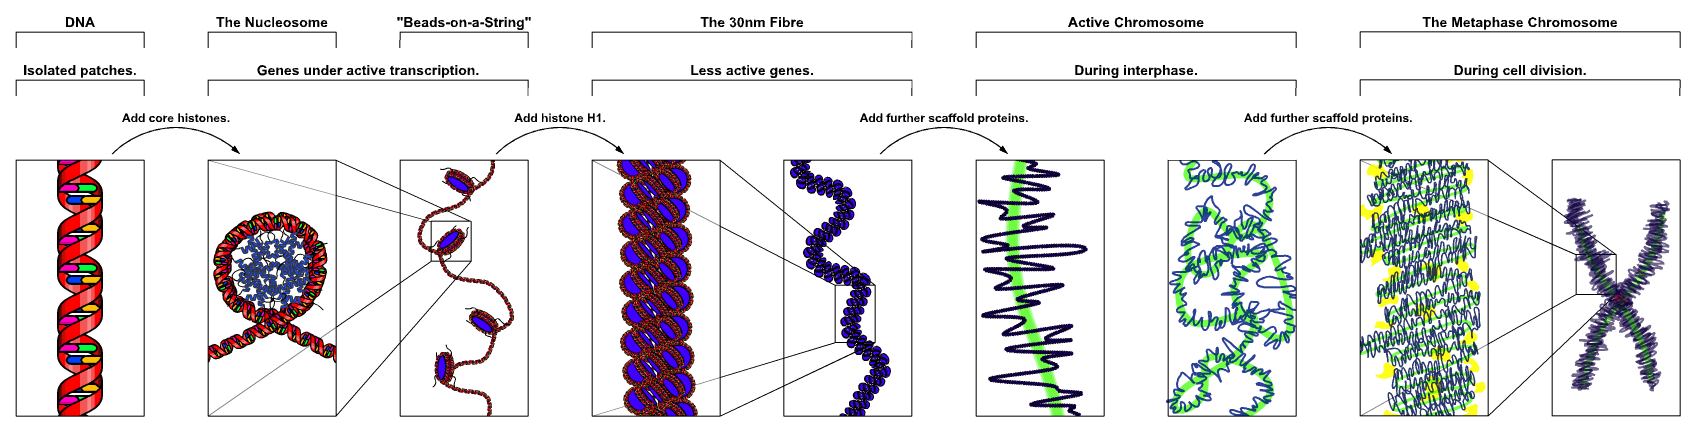
\includegraphics[scale=0.35,trim=15 0 975 155,clip]{Chromatin_Structures}} \\
%     {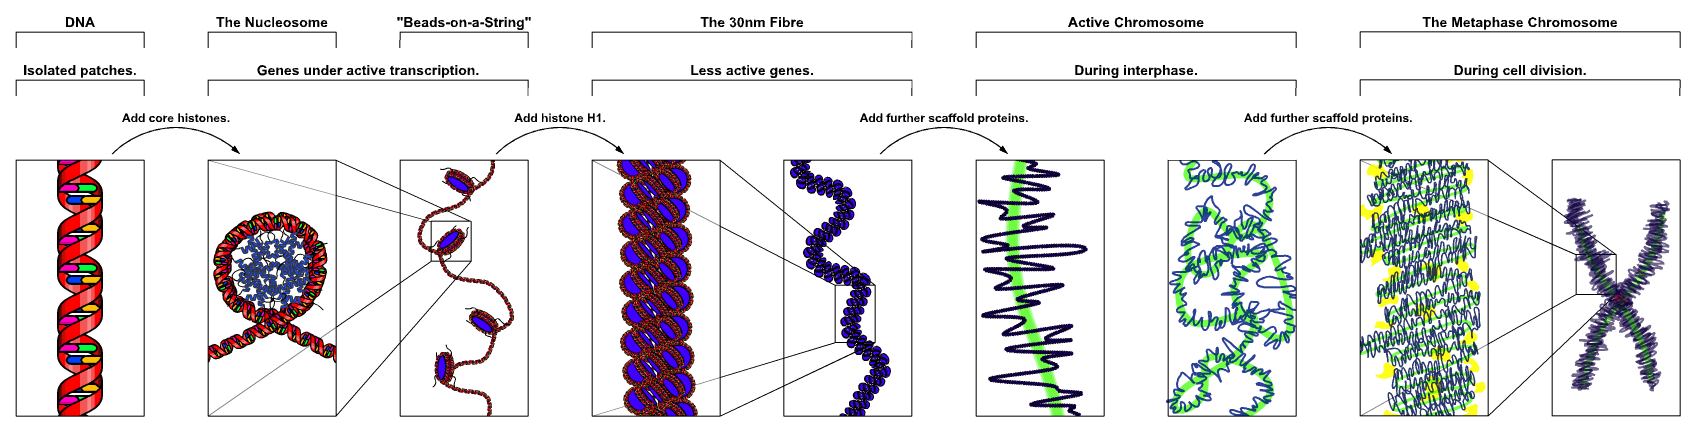
\includegraphics[scale=0.35,trim=784 0 207 155,clip]{Chromatin_Structures}} \\
%     Image adapted from \cite{figchromatinstructures}.
%
% \end{frame}


% \begin{frame}[c]{Spatial Structure}
%     \vfill
%     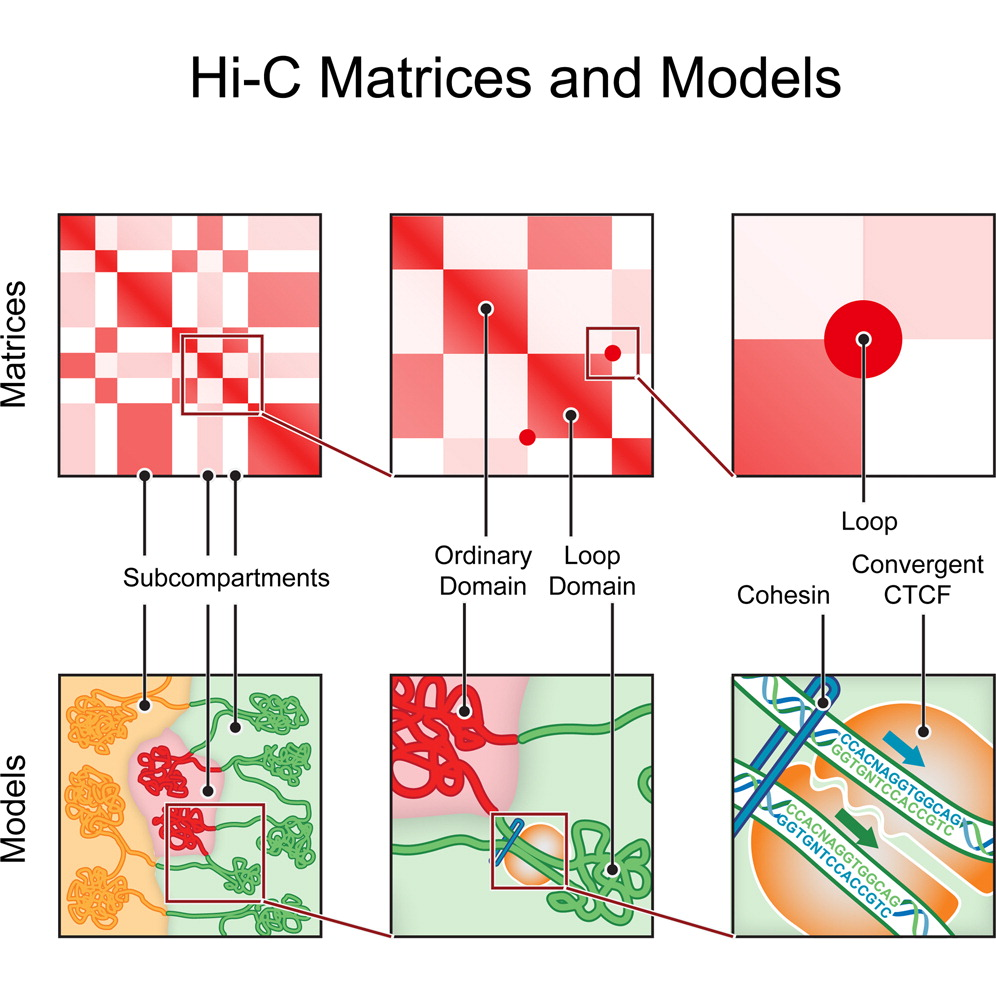
\includegraphics[scale=1.5,trim=0 0 82 130,clip]{HiCMatricesModels} \\
%     Image adapted from \cite{rao20143d}.
% \end{frame}


% \begin{frame}[standout]
%     \Large
%     Enhancers may act on genes from other chromosomes
%     \cite{spilianakis2005interchromosomal}!
% \end{frame}





% Inhalt Vortrag:
% - Kurze motivation was man da machen will
% - Hi-C, grobe Erklärung was da passiert
% - Algorithmus selbst im Detail
% - Implementation ein paar erkenntnisse / schmankerl
% - Resultate
